\subsection{Business Logic Layer}
ViewModels ligger som en mellemting mellem business logic layer og presentation layer. Der foregår en binding til fra viewsne til dataen i viewmodels.

\subsection{Business Logic Layer}
ViewModels ligger som en mellemting mellem business logic layer og presentation layer. Der foregår en binding til fra viewsne til dataen i viewmodels.

\subsubsection*{Viewmodel kommunikation}
Alle view startes fra MainViewViewModel, som invidviduelt starter deres egen viewmodel. Det betyder at det ville være nødvendigt at lave data globalt for at kunne arbejde på den samme data, som f.eks. kategorier og de individuelle produkter i disse. \\
For at løse dette, har vi valgt at bruge Prism EventAggregator~\cite{PRISM}, som tillader os at kommu-nikere på tværs af viewmodels. Når MainViewViewModel startes, subscriber den på en række forskellige events, som bliver rasied når følgende vinduer bliver loaded:

\begin{itemize}
\item AddProductWindow
\item AddCategoryWindow
\item EditProductWindow
\item EditCategoryWindow
\item DeleteCategoryWindow
\end{itemize}


MainWindowViewModel har da en metode for hver af disse events, som bliver kaldt når disse events bliver rasied. Når dette sker publisher MainWindowViewModel så et event, svarende til det vindue der er blevet loaded. Eksempelvis vil AddCategory’s eventhandler publishe et event som AddCate-goryWindow subscriber på, med alle de nuværende kategorier som en parameter.\\

På denne måde undgår vi da, at der skal sendes data ind i et view, og videre ned i en viewmodel. Hvis der er brug for mere end en parameter, eksempelvis EditProduct som skal bruge fire parametre, er det nødvendigt at lave sin egen parameter-type for dette  (Backend.Models.Events : Parameters).

\begin{figure}[!h]
    \centering
    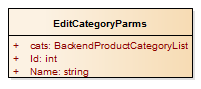
\includegraphics[width=0.3\textwidth]{Systemdesign/backend/Images/parms.png}
    \caption{Eksempel på parametermodel, der i dette tilfælde er til når EditProductViewet bliver loaded}
    \label{fig:editparms}
\end{figure}



\subsubsection{Viewmodel kommunikation}
Alle view startes fra MainViewViewModel, som invidviduelt starter deres egen viewmodel. Det betyder at det ville være nødvendigt at lave data globalt for at kunne arbejde på den samme data, som f.eks. kategorier og de individuelle produkter i disse. \\
For at løse dette, har vi valgt at bruge Prism EventAggregator~\cite{PRISM}, som tillader os at kommu-nikere på tværs af viewmodels. Når MainViewViewModel startes, subscriber den på en række forskellige events, som bliver rasied når følgende vinduer bliver loaded:

\begin{itemize}
\item AddProductWindow
\item AddCategoryWindow
\item EditProductWindow
\item EditCategoryWindow
\item DeleteCategoryWindow
\end{itemize}


MainWindowViewModel har da en metode for hver af disse events, som bliver kaldt når disse events bliver rasied. Når dette sker publisher MainWindowViewModel så et event, svarende til det vindue der er blevet loaded. Eksempelvis vil AddCategory’s eventhandler publishe et event som AddCate-goryWindow subscriber på, med alle de nuværende kategorier som en parameter.\\

På denne måde undgår vi da, at der skal sendes data ind i et view, og videre ned i en viewmodel. Hvis der er brug for mere end en parameter, eksempelvis EditProduct som skal bruge fire parametre, er det nødvendigt at lave sin egen parameter-type for dette  (Backend.Models.Events : Parameters).

\begin{figure}[!h]
    \centering
    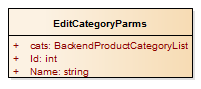
\includegraphics[width=0.3\textwidth]{Systemdesign/backend/Images/parms.png}
    \caption{Eksempel på parametermodel, der i dette tilfælde er til når EditProductViewet bliver loaded}
    \label{fig:editparms}
\end{figure}
